\chapter{Design}

This chapter describes the design process for this project. Initially, the concept of the product is presented with the storyboard to explain the product of the project. The product is then shown and described with the sketches and the iterations that the product went through in the project. Next a walkthrough of the mental model lo-fi test together with the affordance scheme and the results of the test. In the end of the chapter, the design choices for the product are discussed and a conclusion for the chapter.

\section{Concept}
The concept of the product is to be able to apply voice effects in real-time without using a panel or have someone backstage do it for you. The idea is based on giving the singer/performer more freedom and control over how they want to sound in a natural way, compared to turning knobs or using sliders. Most singers always have their hands available, therefore the concept is based on a controller based on hand movement. The hand movement would be different gestures to control which effect to apply and the degree of it.
The controller would implement a gyroscope to sense the hand and wrist movement. The chosen gesture is based on which two fingers the user connects. The index- or middle finger each control their own effect when the finger is connected to the thumb.
The two original ideas for voice effects were pitch shift and reverb. Reverb was later changed to harmonization as this effect was more common in the industry.


\begin{itemize}
\item Harmonising: This will be controlled by turning the hand while having thumb and a finger pressed together, like turning a knob or volume control.
\item Pitch: This will be controlled by lifting or lowering the hand while having thumb and a finger pressed together, like pulling a slider up or down.
\end{itemize}

\section{Storyboard}

To understand the concept and how it would work in a real scenario a storyboard was created to explain how, what and where to use the product, see figure \ref{Storyboard1}. this storyboard was part of the proof of concept that together with the initial sketches would explain the idea better.\\

\begin{minipage}{\linewidth}% to keep image and caption on one page
\makebox[\linewidth]{%        to center the image
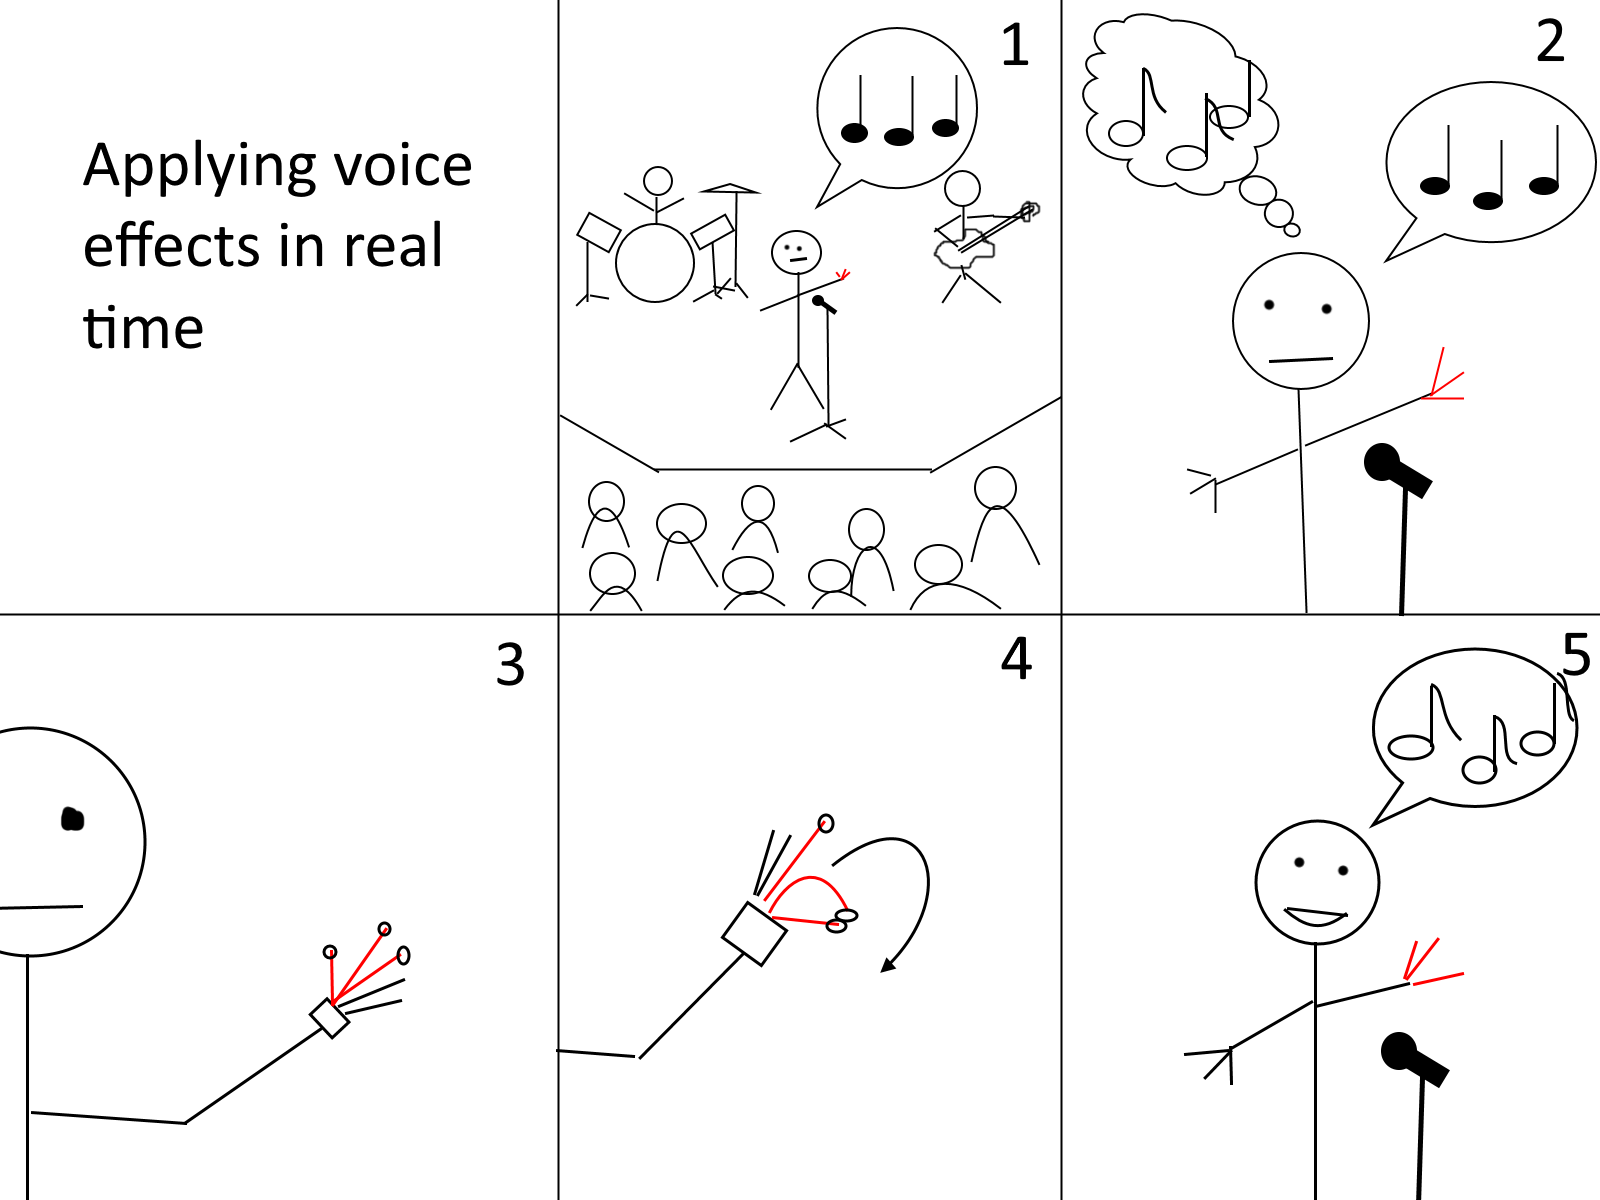
\includegraphics[keepaspectratio=true,scale=0.3]{Storyboard2}}
\captionof{figure}{The Storyboard}\label{Storyboard1}
\end{minipage}\\

In the first frame a band is shown playing a concert on a stage, with the lead singer singing. The seond frame shows the lead singer singing, but wanting to sound different. In the third frame the device is shown on the singer's hand. Fourth frame illustrates the singer performing a gesture to apply the desired effect. The final frame then shows the singer sounding how they wanted to sound.

\section{Sketching and Testing}

The initial sketches and the first concrete design of the device have copper foil on thumb, index finger and middle finger, see figure \ref{Sketch1}. When pressing the index or middle finger together with the thumb, a connection is made in the system that activates the assigned effect. \\

\begin{minipage}{\linewidth}% to keep image and caption on one page
\makebox[\linewidth]{%        to center the image
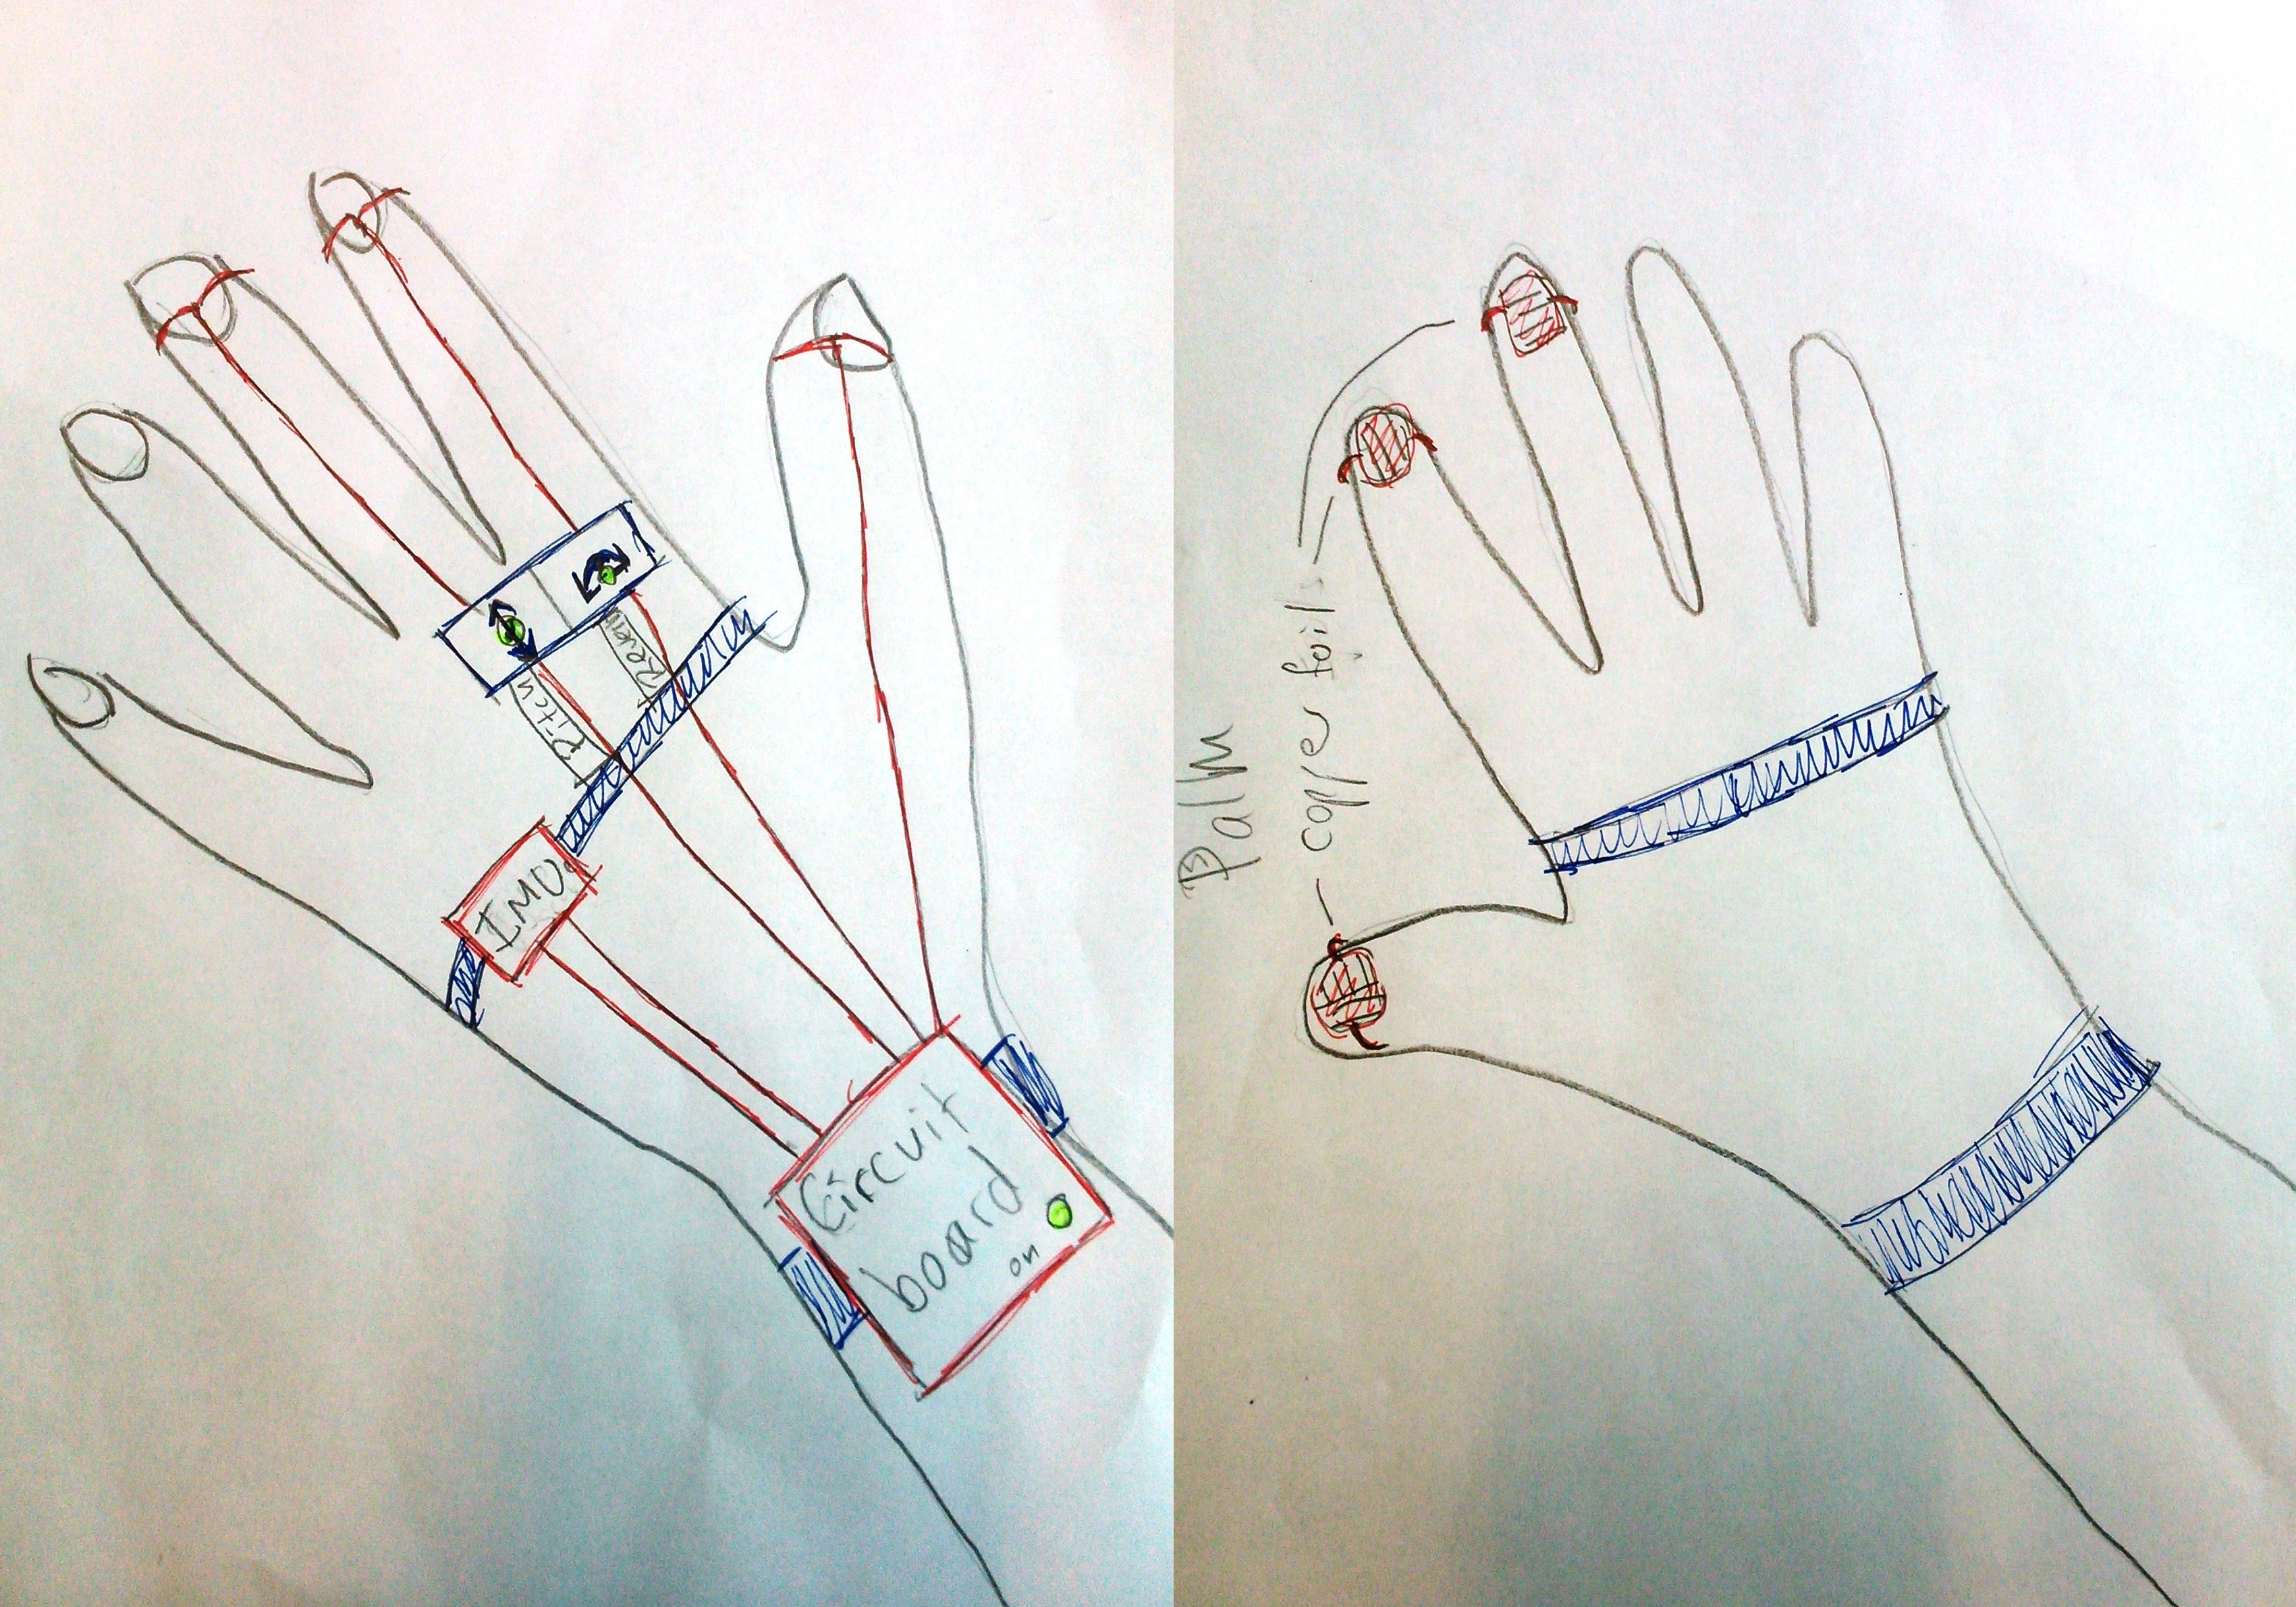
\includegraphics[keepaspectratio=true,scale=0.1]{Sketch1}}
\captionof{figure}{Two sketches showing idea of the system}\label{Sketch1}
\end{minipage}\\

On the knuckles there are illustrations of the gestures, that you are supposed to do to manipulate the effects. Beneath those are small labels with the name of the effect. In this design reverb is used instead of harmonising. This was later changed, since reverb is not manipulated quite as much as harmonising.

The sensor is attached to the hand by a velcro strip, as is the circuit board. \\

A quick informal test with three participants was conducted and they were told what the drawing was supposed to be and what it should do. They then had to figure out based on the sketch how to do those things.
From this test, a few key things were learned:
 
\begin{itemize}
	\item They all had difficulty figuring out how to get to the activate stage. None of them connected their fingers.
	\item Most eventually figured out which type of gesture in general had to be done, but only after some trial and error
	\item They all found out which finger created which effect
\end{itemize}

Based on that the next focus was on creating some feedforward and perceived affordance that tells the user, that to activate the glove you need to connect two fingers.

The second sketch changed the illustrations since people had a hard time immediately recognising the correct gestures with the old ones, as seen in figure \ref{Sketch2}.\\

\begin{minipage}{\linewidth}% to keep image and caption on one page
\makebox[\linewidth]{%        to center the image
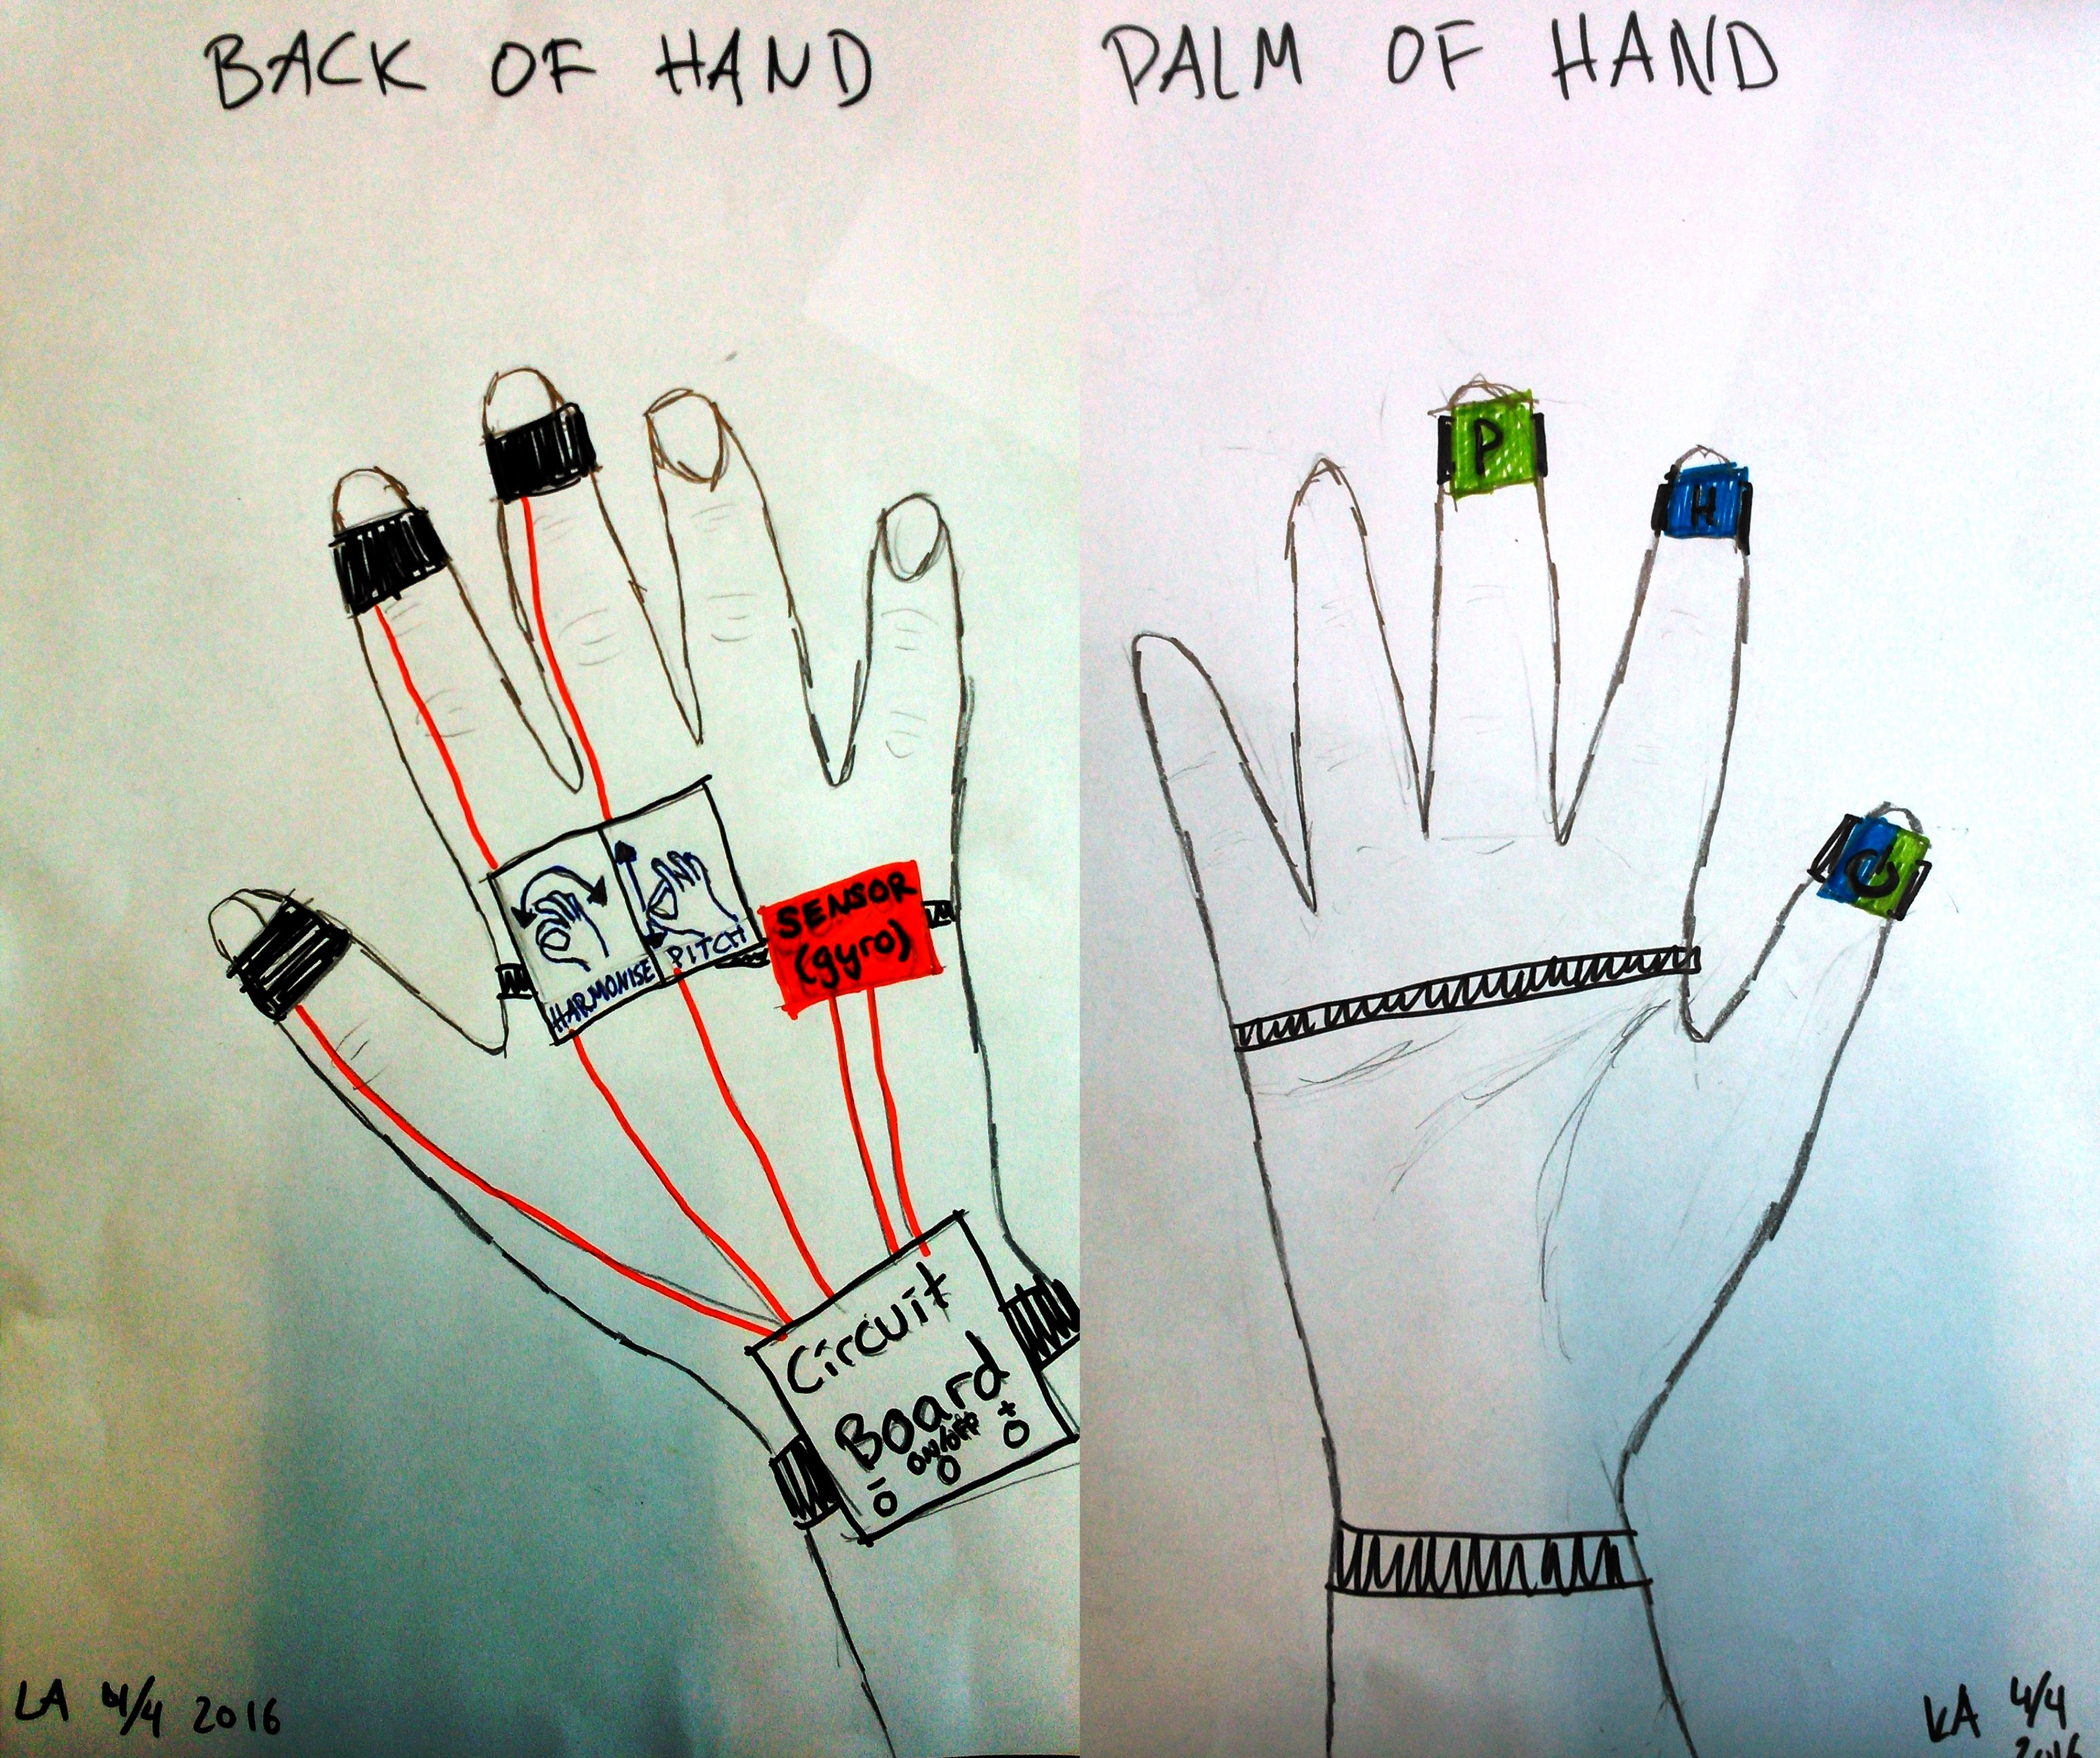
\includegraphics[keepaspectratio=true,scale=0.1]{Sketch2}}
\captionof{figure}{Second set of sketches after some changes}\label{Sketch2}
\end{minipage}\\

Colour was also added to the copper foil, a different one on the index and middle finger and then both on the thumb. This was done to create perceived affordance between the fingers and thumb.

LEDs were added on the circuit board to create some feedback for the actions. The middle LED showing if the system was on or off. The two other LEDs showing an increase or decrease in the effect, with a minus and a plus sign.\\

A quick informal test was done with two participants with the revised sketch. Now there was a better indication that they needed to connect two fingers, but not anything that indicated that they needed to stay connected.
Additional results from the test:

\begin{itemize}
	\item One suggested that instead of the on/off LED, maybe a connected/not connected LED.
	\item The arrows were found to be confusing for one tester.
	\item Another tester easily understood the pitch action but was a bit confused with the placement of the arrow on the harmonise action.
	\item One tester thought tht the dual colour on the thumb suggested that both actions could be done at the same time.
	\item The plus and minus LEDs confused one tester, but this could also be because the drawing was unclear.
\end{itemize} 

\section{Lo-Fi}

Based on the previous test, a new design iteration of the glove was made, now also in the form of a lo-fi model, as seen in figure \ref{LoFiHand}. This lo-fi was created in order to make a mental model test. The desire was to both get some feedback on the general design, but also to weigh the users' mental model against an affordance scheme.\\

\begin{minipage}{\linewidth}% to keep image and caption on one page
\makebox[\linewidth]{%        to center the image
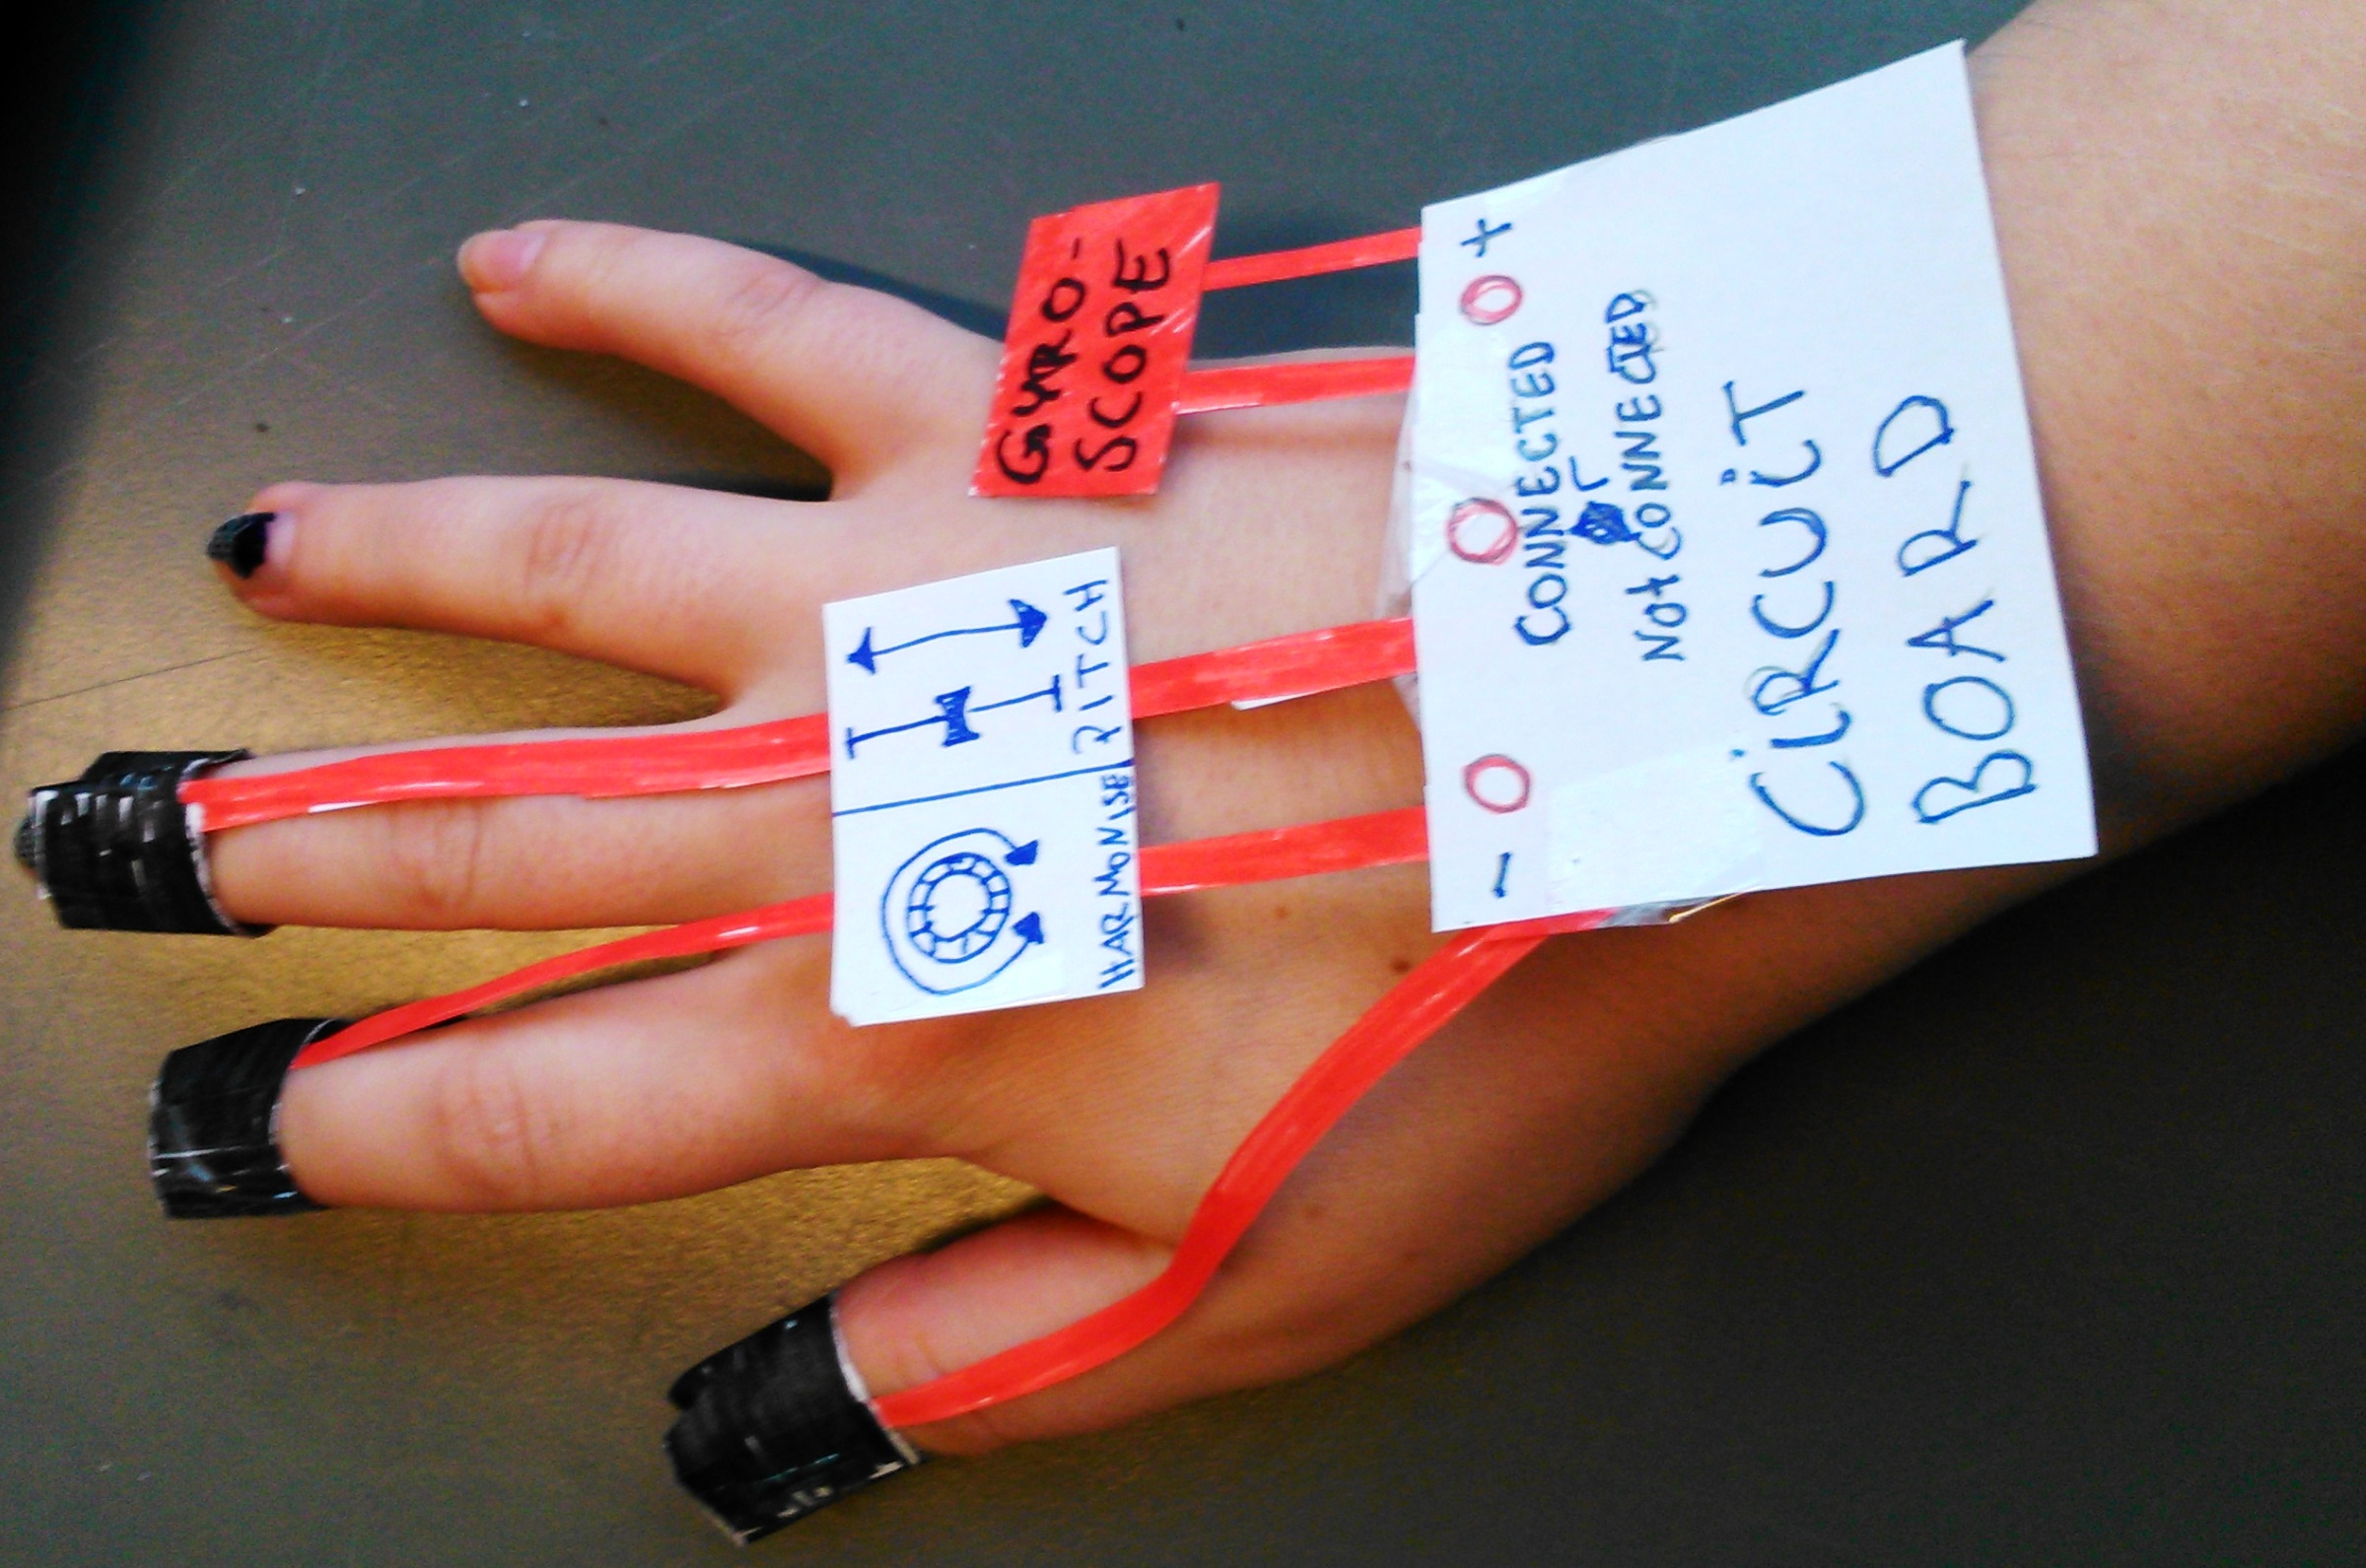
\includegraphics[keepaspectratio=true,scale=0.1]{LoFiHand}}
\captionof{figure}{The Lo-fi of the system}\label{LoFiHand}
\end{minipage}\\

\subsection{Affordance Scheme}
The affordance scheme is separated into three categories: perceived affordance, feedforward, and feedback. Perceived affordance is the perception that something is interactable, e.g. a user would assume a button can be pressed no matter what state the system is in. Feedforward is what is expected to happen after a certain action, e.g. after pressing the "On" button, the system will turn On. Finally, feedback is what the system does to indicate an action has taken place, e.g. after pressing the "On" button, a display lights up and says "Turning On".

The following table shows the affordance scheme for the system.

\newcolumntype{c}[1]{>{\centering\let\newline\\\arraybackslash\hspace{0pt}}m{#1}}

\begin{center}
  \begin{tabular}{| c{2cm} | c{3cm} | c{3cm} | c{3cm} |}
    \hline
    \textbf{State} & \textbf{Perceived Affordance} & \textbf{Feedforward} & \textbf{Feedback} \\ \hline
    \textbf{Inactive} & It is a wearable glove & & All LEDs are OFF \\ \hline
    \textbf{Active} &  & Connect fingers + perform gesture on labels = effect change & "Connected" LED is ON \\ \hline        
    \textbf{Performing Gesture} &  & Connect fingers + perform gesture = effect change & Voice Changes and the plus and minus LEDs light accordingly \\ \hline
  \end{tabular}
\end{center}

\subsection{The Test}

The test was initiated with a short introduction for the user, without revealing too much. Then the participants were asked to explain everything they saw and assumed about the glove, and to try to put it on. Following this, they were given the tasks of turning harmonisation up and pitch down. Finally, some follow-up questions were asked to figure out why they did what they did.

Seven people participated in the test. Here are some results from the test:

\begin{itemize}
	\item When trying to apply the effects, 6 out of 7 testers' first reaction was to not connect their fingers
	\item 5 out of 7 did the correct gestures, based on the ilustrations on the knuckles
	\begin{itemize}
		\item 1 of the two who did not do the correct gestures, did what she did because she thought the illustrations were interactable
	\end{itemize}
	\item 6 out of 7 found the illustrations helpful
	\item All participants figured out that the device was a glove to wear on the hand
	\begin{itemize}
		\item 5 out of 7 put it on correctly, as seen in figure \ref{LoFiHand}
	\end{itemize}
	\item All participants were in doubt of what the LEDs were for
\end{itemize}

The table below shows a revised affordance scheme based on the user feedback. The parts of the system that the participants had a hard time understanding are shown in red writing in the table. Additionally, the parts which were generally understood by the users has the text coloured green.

\begin{center}
  \begin{tabular}{| c{2cm} | c{3cm} | c{3cm} | c{3cm} |}
    \hline
    \textbf{State} & \textbf{Perceived Affordance} & \textbf{Feedforward} & \textbf{Feedback} \\ \hline
    \textbf{Inactive} & \textcolor{green}{It is a wearable glove} & & \textcolor{red}{All LEDs are OFF} \\ \hline
    \textbf{Active} &  & \textcolor{red}{Connect fingers} + \textcolor{green}{perform gesture on labels} = effect change & \textcolor{red}{"Connected" LED is ON} \\ \hline        
    \textbf{Performing Gesture} &  & \textcolor{red}{Connect fingers} + \textcolor{green}{perform gesture} = effect change & \textcolor{red}{Voice Changes and the plus and minus LEDs light accordingly} \\ \hline
  \end{tabular}
\end{center}

The participants had a hard time understanding some of the feedback in the system, particularly the LEDs. While they knew that they were LEDs, they were not sure what each of them was signifying. This could also be a result of bad simulation of the LED state changes in the test.
Another thing that the users had a hard time understanding was the colour coding on the fingers. Most did not connect their fingers to initiate the effect change.

The things that the users perceived correctly was that the system was to be used as a glove. After the alterations based off of earlier tests, the new illustrations had much more success regarding the gestures. Most understood the feedforward provided by the labels and performed the gesture correctly, although without connecting the fingers.

\section{Design Choices}

Throughout the design process a lot of choices have been made regarding the design of the system. The reasoning behind these decisions will be discussed in this section.\\

Very early on in the process, it was decided to make the gestures base off of some gestures that people would normally associate with manipulating music, like a volume knob or a slider on an equalizer, as seen in figure \ref{SynthAmp}.\\

\begin{minipage}{\linewidth}% to keep image and caption on one page
\makebox[\linewidth]{%        to center the image
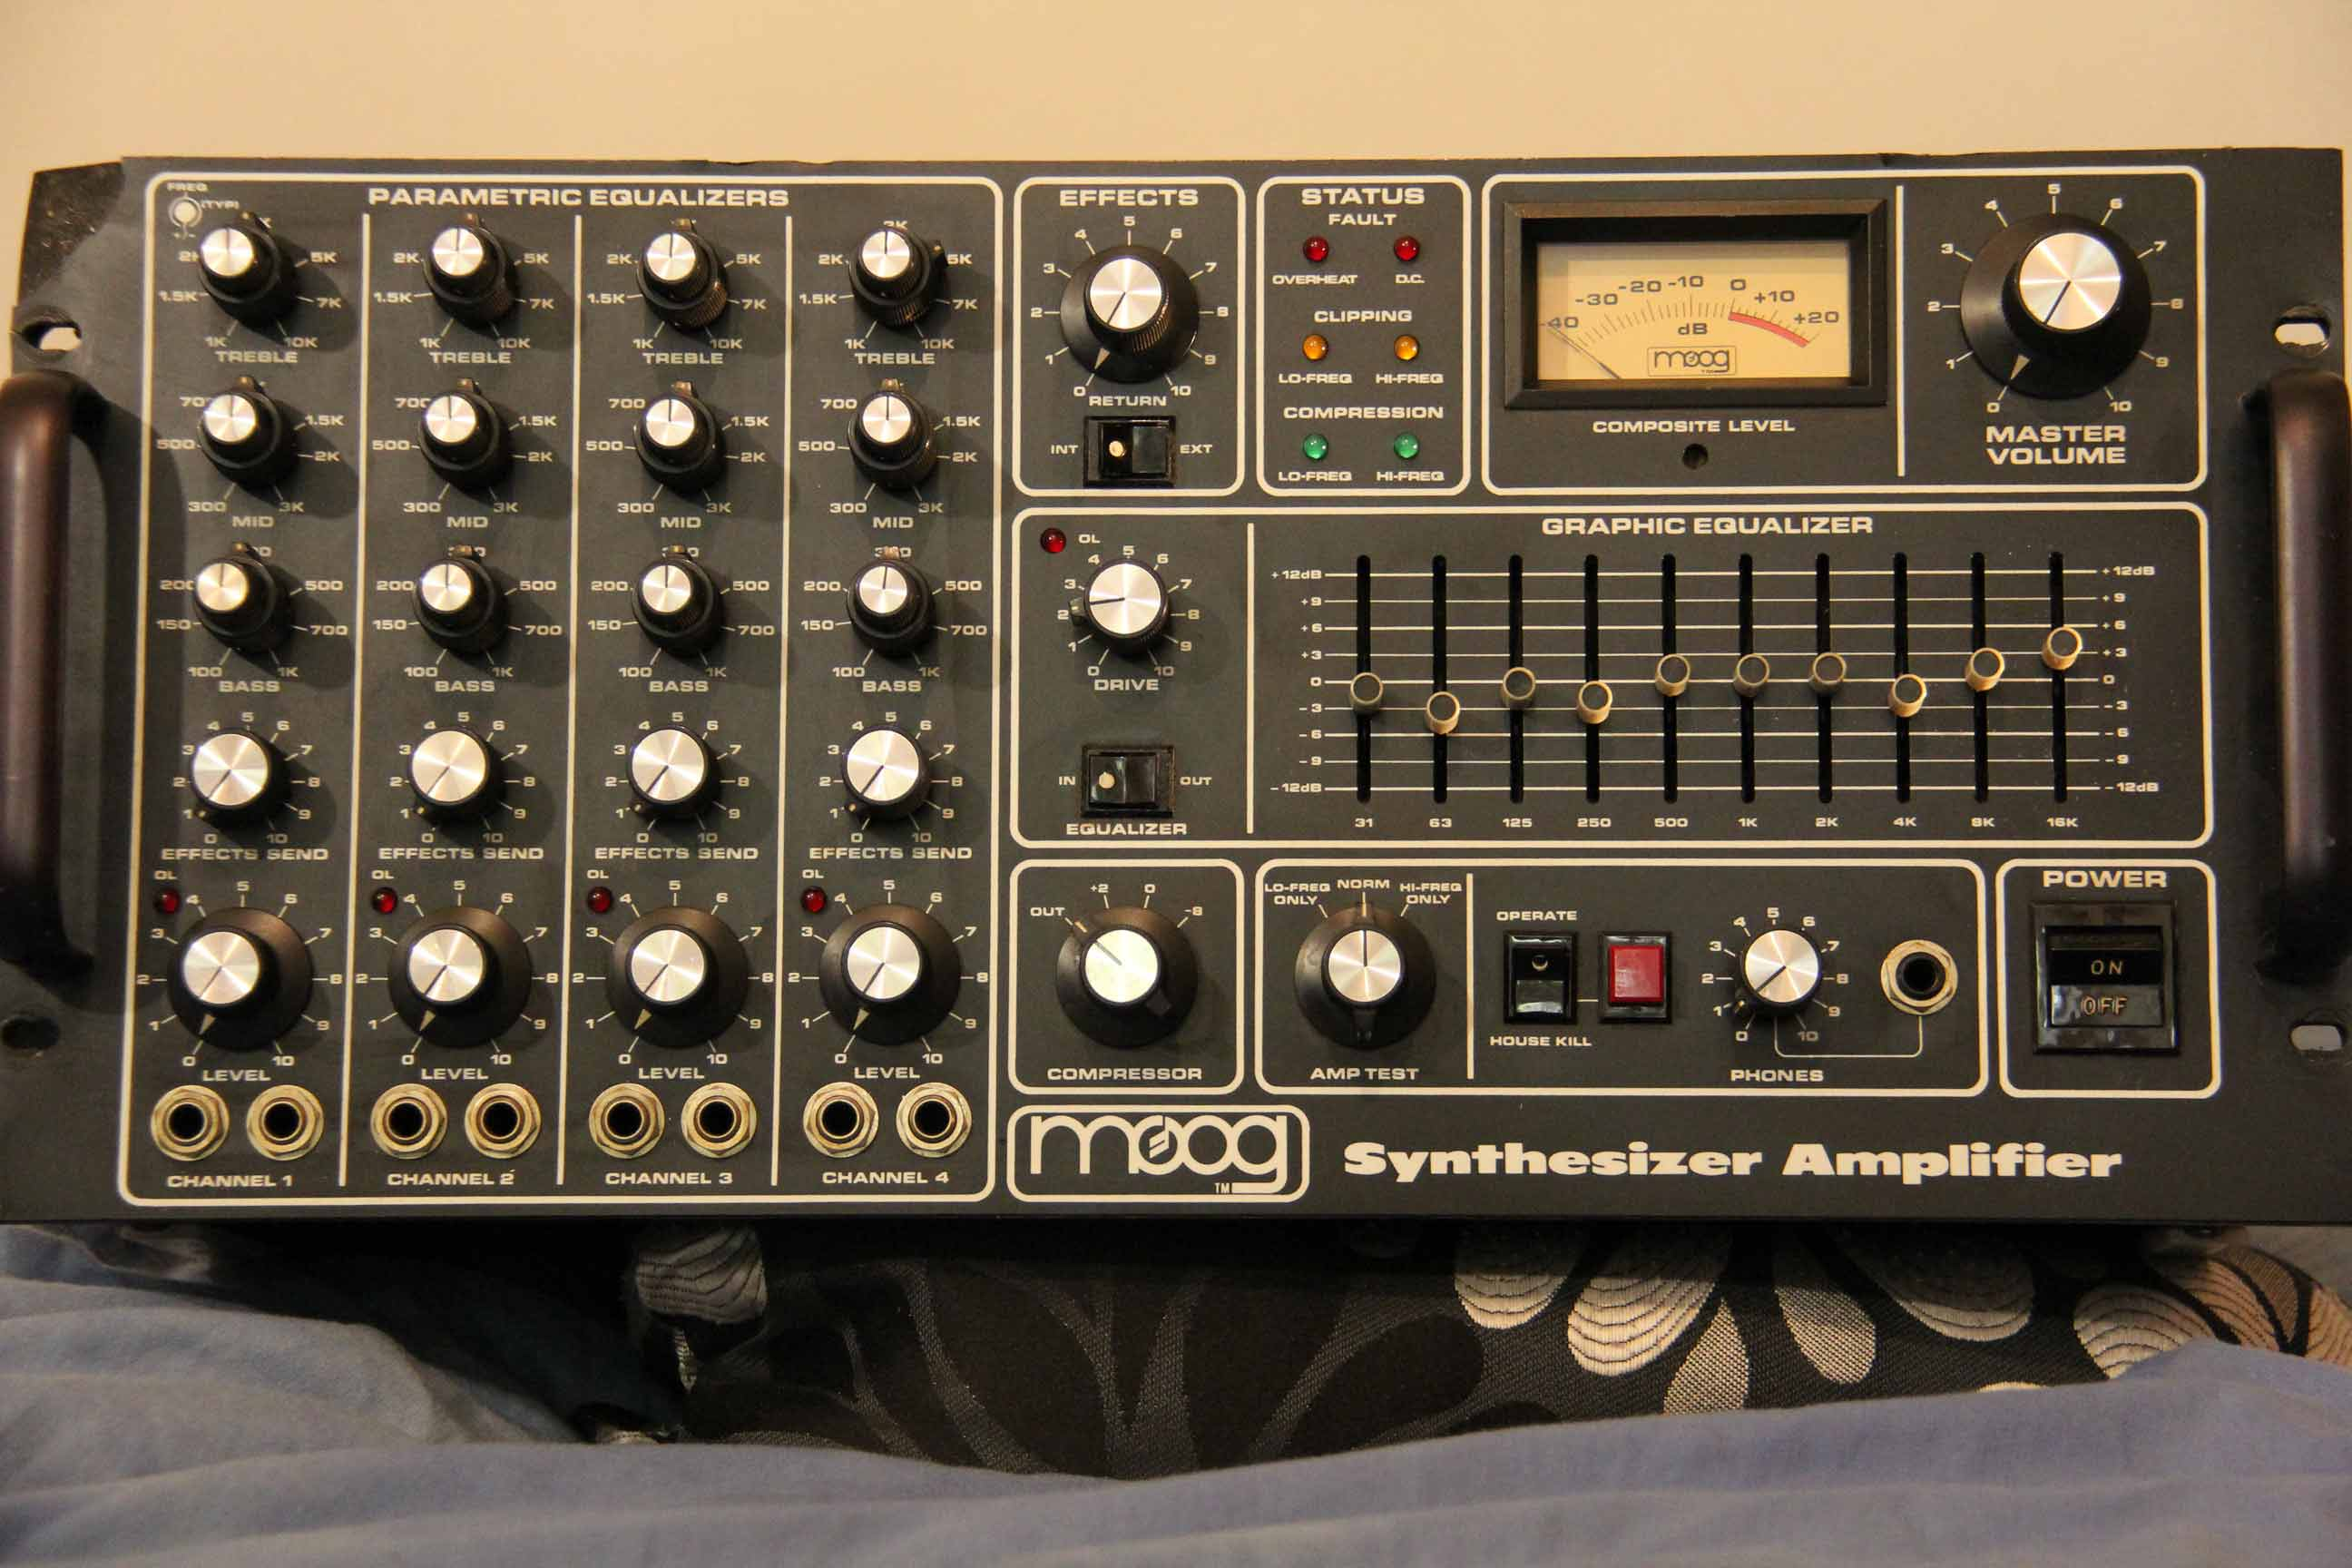
\includegraphics[keepaspectratio=true,scale=0.1]{SynthAmp}}
\captionof{figure}{The AX 301 Synthesizer Amplifier with knobs and sliders\citep{AudioFan}}\label{SynthAmp}
\end{minipage}\\

The gesture of turning a knob was assigned to the harmonize effect, while the vertical slider gesture was assigned to the pitch shift. Since pitch shift is manipulated by making a higher or lower pitch, it makes sense to make the gestures simulate a vertical slider, with a higher pitch being assigned to moving up, and lower pitch assigned to moving down.
Furthermore, in accordance to the "turning a knob" and "moving a slider" sentiment, it had to be implemented on the actual glove. This was done by adding some copper band on some velcro for the fingers. This copper was then connected to the circuit board with wires. When connecting the fingers, this would then allow the corresponding effect to be activated, and then the effect could be changed by using the gestures.

When looking at the feedback for the glove, other than the voice changing, it was decided to use LEDs as a way to communicate state changes. A red LED was used to indicate that the effects were being changed in the negative direction, e.g. pitch being lowered, and a green LED was used for the positive direction. Additionally, these LEDs would be accompanied by labels. A minus sign for the negative direction and a plus sign for the positive. The red LED and the minus sign would be placed on the left side of the circuit board to indicate the negative direction the "knob" had to move. The green LED and the plus sign would be placed on the right side to indicate the positive direction.
Finally, a yellow LED was placed in the center of the circuit board. This LED will indicate whether the glove was active or not. Active being the state where an effect could be changed.


\section{Conclusion}

The first concept of the system was a glove that uses a gyroscope to sense hand movement, and apply voice filters according to the movement. A storyboard was created to show how the system would be used and in what context. The first sketch showcased the system with copper foils on the fingers, and labels to explain how to operate the device. This sketch included reverb as an effect to apply, which was later changed since reverb is mostly irrelevant for a singer. The second iteration also included new labels to provide better feedforward and LEDs for feedback when interacting with the system. The third iteration once again included new labels, this time with more success and was made into a lo-fi model. This iteration was compared to the affordance scheme with the results showing the labels were better, but the system lacking elsewhere, namely an indication of the connection of the fingers to apply an effect. The test participants also had some trouble understanding the feedback of the system, as in how the LEDs worked and what sort of feedback they actually provided.